% !TEX root =  ../../master.tex
\chapter{Abbildungen}

\begin{figure}[h]
	\centering
	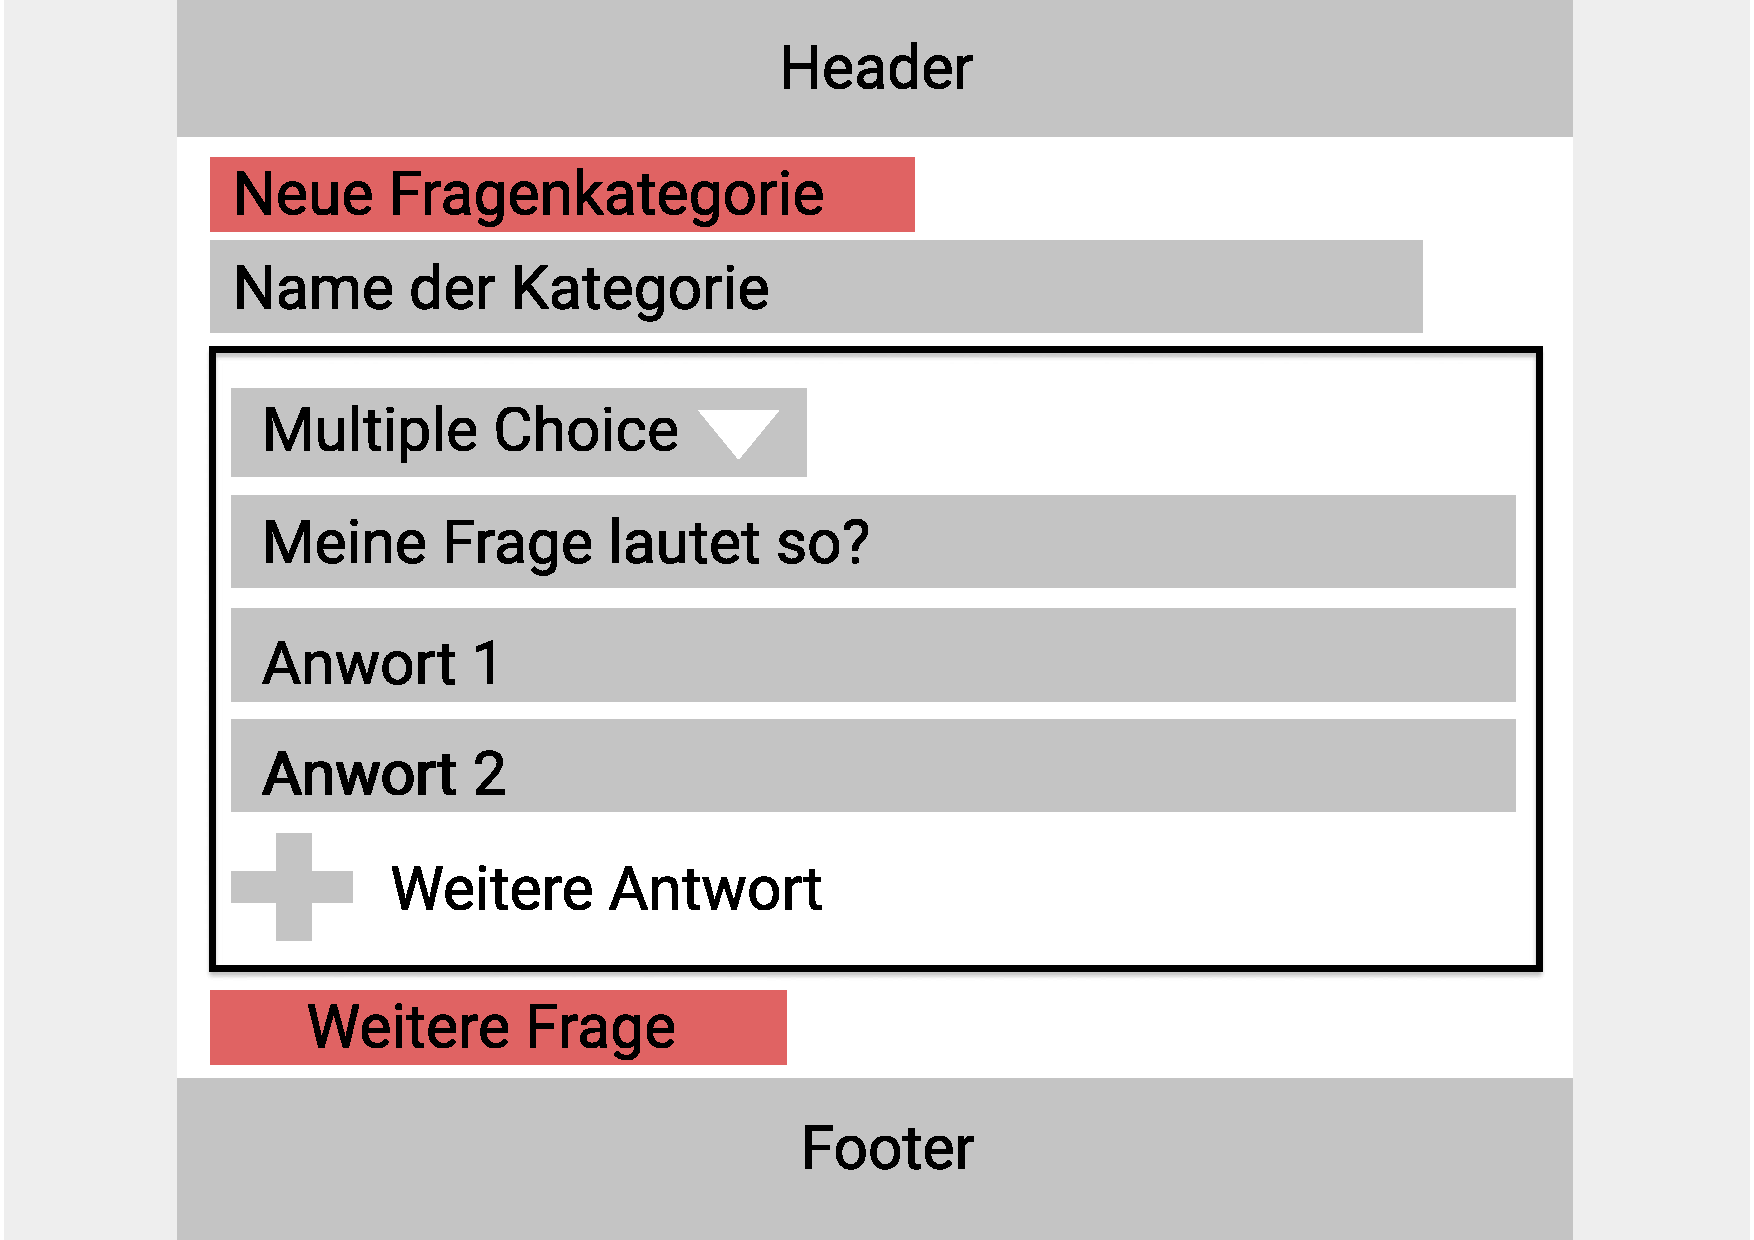
\includegraphics[width=0.7\textwidth]{img/konzeption/client/umfrage_erstellen_multiple_choice}
	\captionsetup{justification=centering, format=plain}
	\caption[Mock-Up der Umfrageerstellung von Multiple-Choice-Fragen]{Mock-Up der Umfrageerstellung von Multiple-Choice-Fragen \\\figma}
	\label{fig:MockUmfrageMultipleChoice}
\end{figure}

\begin{figure}[h]
	\centering
	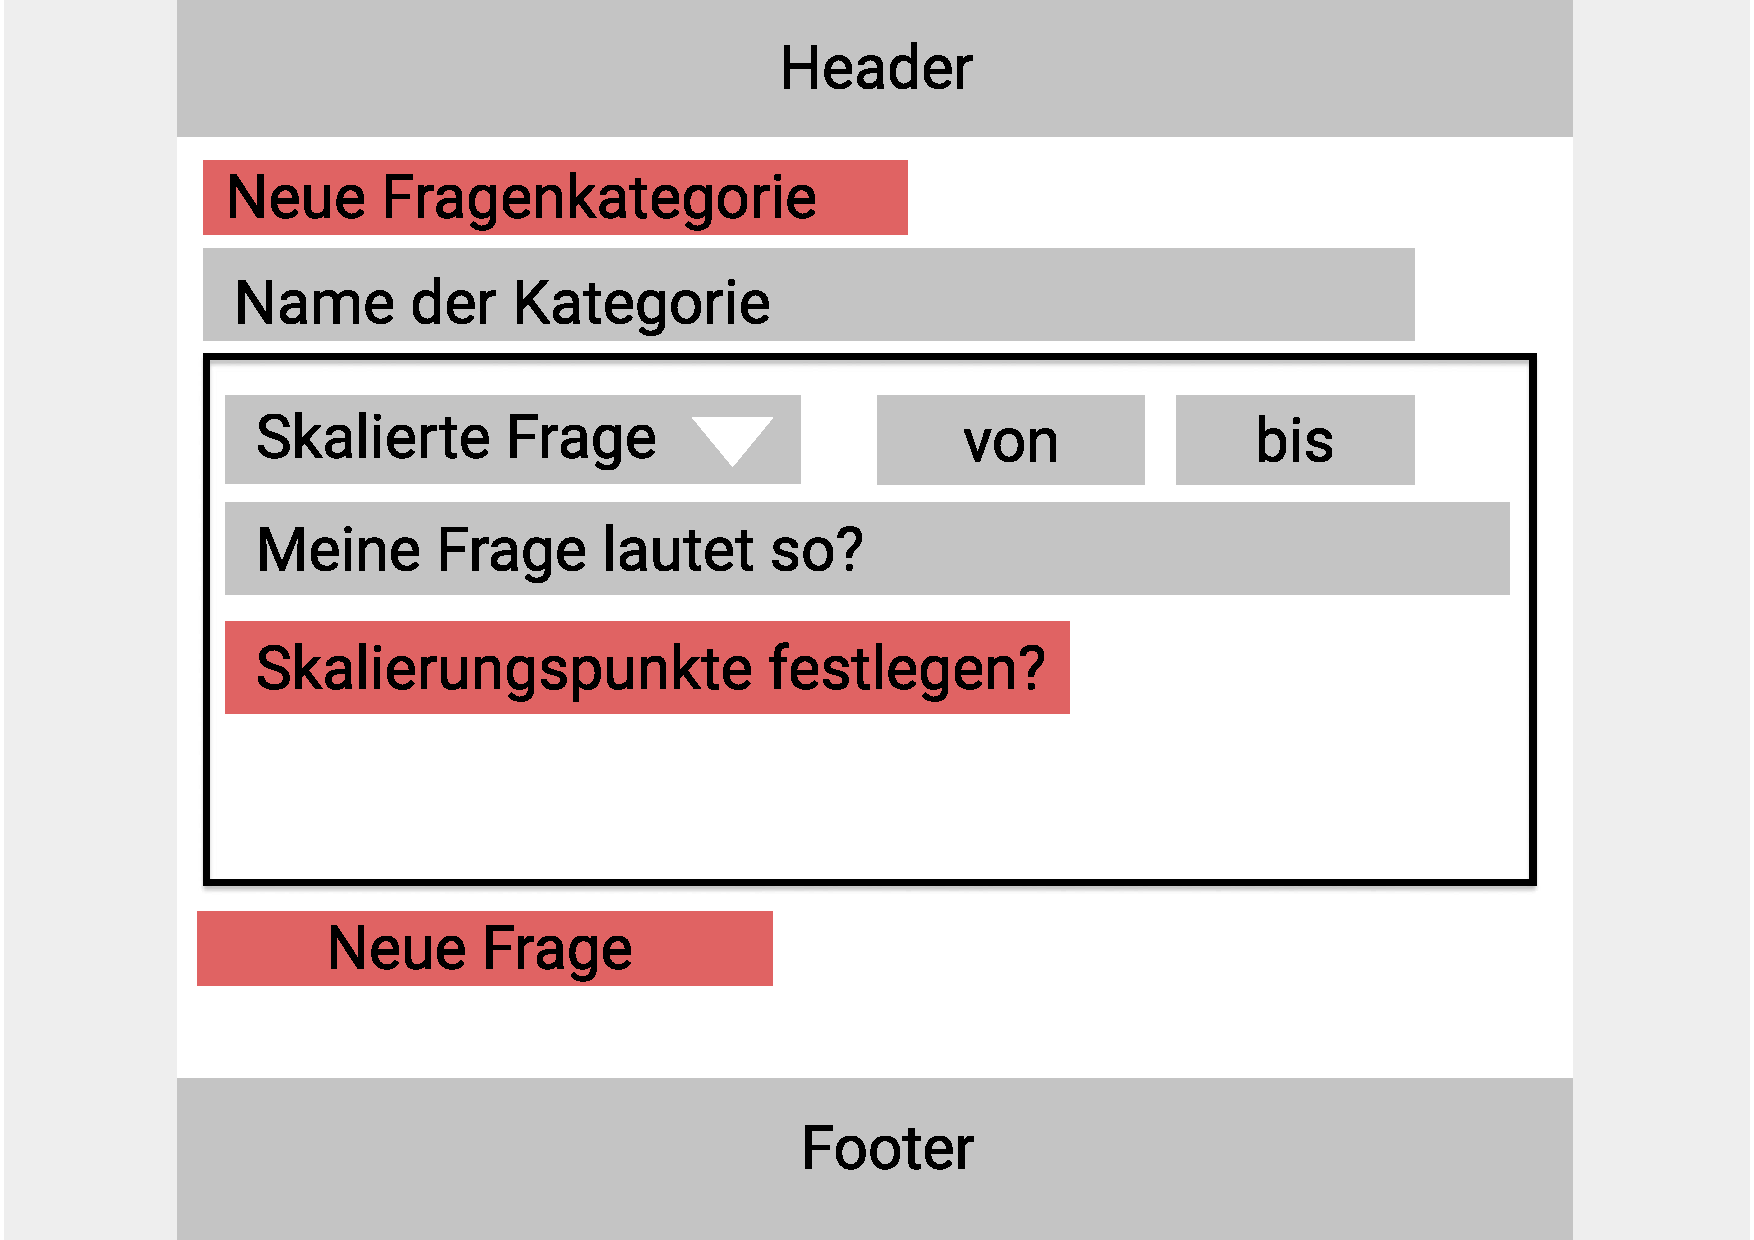
\includegraphics[width=0.7\textwidth]{img/konzeption/client/umfrage_erstellen_rating}
	\captionsetup{justification=centering, format=plain}
	\caption[Mock-Up der Umfrageerstellung von Rating-Fragen]{Mock-Up der Umfrageerstellung von Rating-Fragen \\\figma}
	\label{fig:MockUmfrageRating}
\end{figure}
